\chapter{Definition and motivation of a N/CI}
\label{appendix1-definition-and-motivation-of-a-nci}
\graphicspath{{Appendix1/Figs/}{Appendix1/Figs/}}

This section discusses the definition, need and differentiation of a N/CI and the paradigm shifts associated with it when discussing BCI software.

\section*{BCI software on the cloud}
\label{chapter2-bci-software-on-the-cloud}

Looking at \autoref{fig:nci-components}, we can see that the three software layers of a BCI-component illustration, as pictured on \autoref{fig:bci-components} are highlighted. This is due to the fact that these components are not bound to a physical interface such as a cable or Bluetooth.

\begin{figure}[ht]
  \centering
  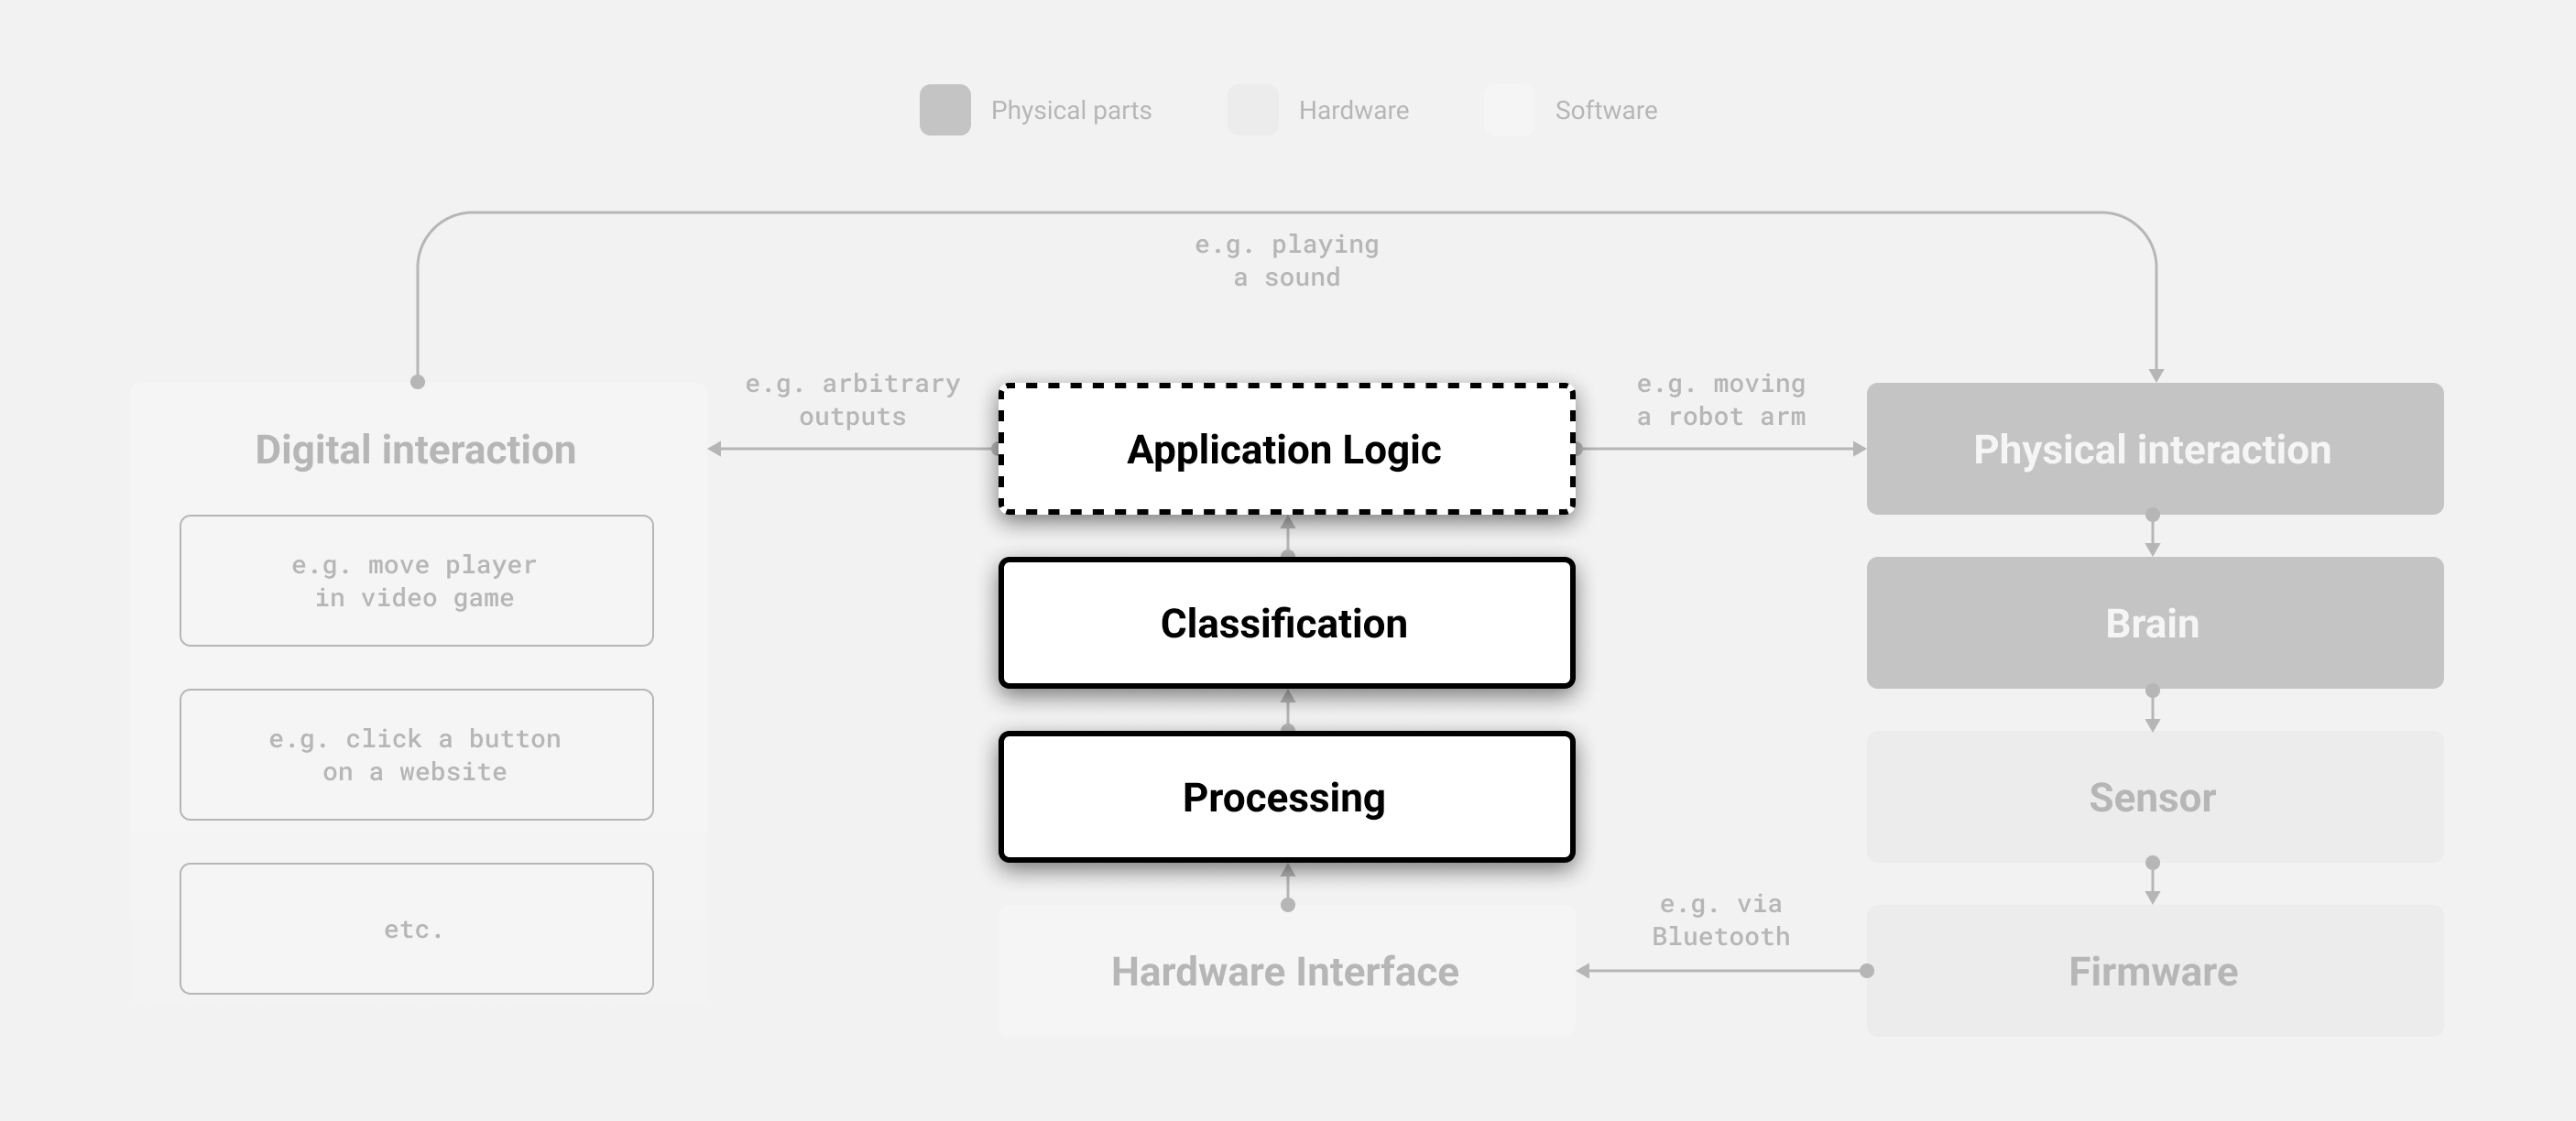
\includegraphics[width=\linewidth]{nci-components.png}
  \caption{Highlighted software components as previously shown on \autoref{fig:bci-components} of a BCI that could be moved to the cloud.}
  \label{fig:nci-components}
\end{figure}

Running software on the cloud means that developers or companies can access provisioned information technology (IT) infrastructure through the internet, usually with a pay-as-you-go pricing model \citep{amazon_web_services_inc_what_nodate}. The development speed of software applications can drastically improve since software developers can only focus on software rather than incorporating the hardware and network aspect of setting up their server farms, therefore abstracting the hardware part away. What started with simple computers that can be rented in a remote server farm such as it was with, e.g. Amazon Web Services (AWS) Elastic Compute Cloud (EC2) \citep{barr_amazon_2006} ended up being a diverse offering from cloud providers with various abstraction levels as shown in \autoref{tab:cloud-computing-types}.

\begin{table}[!ht]
  \centering
  \resizebox{\textwidth}{!}{%
    \begin{tabular}{ll}
      \rowcolor[HTML]{000000}
      {\color[HTML]{FFFFFF} Type}                                                                                 &
      {\color[HTML]{FFFFFF} Description}                                                                                                                                                                                                                                                                                                                           \\ \hline
      \multicolumn{1}{|l|}{\textbf{\begin{tabular}[c]{@{}l@{}}Infrastructure as\\ a Service (laaS)\end{tabular}}} &
      \multicolumn{1}{l|}{\begin{tabular}[c]{@{}l@{}}IaaS gives access to data storage space, virtual or dedicated\\ computers, and network services. The greatest degree of\\ flexibility and administrative control over your IT resources\\ are provided by utilising IaaS.\end{tabular}}                                                                       \\ \hline
      \multicolumn{1}{|l|}{\textbf{\begin{tabular}[c]{@{}l@{}}Platform as a\\ Service (PaaS)\end{tabular}}}       &
      \multicolumn{1}{l|}{\begin{tabular}[c]{@{}l@{}}PaaS lets developers concentrate on developing and\\ managing their code rather than worrying about the\\ underlying infrastructure (often hardware and operating\\ systems). An example is Kubernetes.\end{tabular}}                                                                                         \\ \hline
      \multicolumn{1}{|l|}{\textbf{\begin{tabular}[c]{@{}l@{}}Software as a\\ Service (SaaS)\end{tabular}}}       &
      \multicolumn{1}{l|}{\begin{tabular}[c]{@{}l@{}}SaaS provides a whole product that is run and controlled \\ by the service provider. The phrase SaaS often refers to\\ end-user apps (e.g. web-based email). Developers don't\\ have to be concerned about how the service is handled\\ or whether the underlying infrastructure is maintained.\end{tabular}} \\ \hline
    \end{tabular}%
  }
  \vspace{10pt}
  \caption[The three abstraction levels and types of cloud computing]{The three abstraction levels and types of cloud computing \citep{amazon_web_services_inc_what_nodate}.}
  \vspace{-5pt}
  \label{tab:cloud-computing-types}
\end{table}

The majority of businesses are anticipated to embrace a cloud-first strategy by 2025, according to Milind Govekar, vice president of IT research and consultancy company Gartner, and will not be able to fully implement their digital plans without the usage of cloud-native architectures and technologies \citep{gartner_gartner_nodate}. The impact and importance of cloud computing cannot be underestimated, and its success is also reflected in the annual spending on cloud computing resources, estimated at €474 billion in 2022 \citep{gartner_gartner_nodate}. Cloud computing is such an extensive and complex topic that it could quickly fill entire books. The author categorises three broad but essential points that certainly play a vital role in BCI software: 1. Dedicated and deterministic environments, which explains that an environment of a software programme always stays the same independent of the end-users hardware, 2. elastic and high-performance availability, which explains cloud computers that have an on-demand and adjustable high-performance and 3. provided services for speed, which explains the concept of pre-made and dedicated software written primarily for the cloud and specific use cases. The following list goes more into detail about the mentioned topics in the context of BCI software:

\begin{enumerate}
  \item \textbf{Dedicated and deterministic environments:} Running code for BCIs on different end-user platforms, such as Windows or Android, can have drawbacks because each device has its processor, graphics card, operating system version and drivers, which can make developing software that requires stable and good performance, such as neural data processing pipelines, time-consuming and difficult to maintain, as developers must keep track of every factor of the end-user devices. This is fine for BCIs that are not intended for the general public, such as specially designed BCIs for people with, say, locked-in syndrome, but for the general public, a vast amount of different end-user devices could come into play. When code runs on a dedicated machine, such as a cloud computer with clearly defined hardware and operating system specifications, it becomes less error-prone and more deterministic.
  \item \textbf{Elastic and high-performance availability:} Because the cloud usually runs as an as-needed model, the initial purchase cost of computer hardware is split and shared across usage. Developers have access to tremendous computing power that would not be easily afforded if purchased independently. As a result, when developing a computationally intensive algorithm, developers can use high-performance central processing units (CPUs) and graphics processing units (GPUs) to complete tasks much faster than consumer hardware on end-user devices. Performance can also be increased as needed, e.g. to handle computationally heavier tasks that are not used as frequently or to handle more requests when, e.g. the demand for the software increases due to an increase in the number of users, which is a process known as elasticity \citep{gartner_definition_nodate}. Furthermore, the cloud provides far more storage capacity than end-user devices.

  \item \textbf{Provided services for speed:} The vast majority of cloud providers are providing more specialised services as we move closer to PaaS. Provisioned database servers, for example, exist solely to serve as a database, so the underlying hardware is optimised for the database software running on it. Hundreds of cloud computing services are available, including 200 from AWS alone \citep{amazon_web_services_inc_what_nodate}, all of which address specific use cases. This is extremely useful when it comes to cloud-based BCI software. One example is the aspect of live streaming of brain data, which we will go over in greater detail in the implementation chapter of this thesis. The services accelerate development speed by eliminating the need for teams to reinvent the wheel repeatedly, next to also providing out-of-the-box scalability due to built-in elasticity and the concept of fully abstracted hardware via the serverless model  \citep{redhat_what_2022}.
\end{enumerate}

A N/CI utilises cloud computing by running certain software components of a BCI system in the cloud with the benefits as mentioned before. Multiple BCIs can communicate with each other or with other software or hardware over the internet, enabling remote human-computer interaction. \autoref{fig:nci-overview} depicts how two or more BCIs can interface with one another using cloud software. The red arrows represent the typical local BCI. The blue arrow depicts how BCI B  can execute business logic via the cloud over the internet, enabling digital and physical interactions with, e.g. high performance. The green arrow depicts how BCI A can communicate via a N/CI with BCI B even if they are not in the same geographical location.

\begin{figure}[ht]
  \centering
  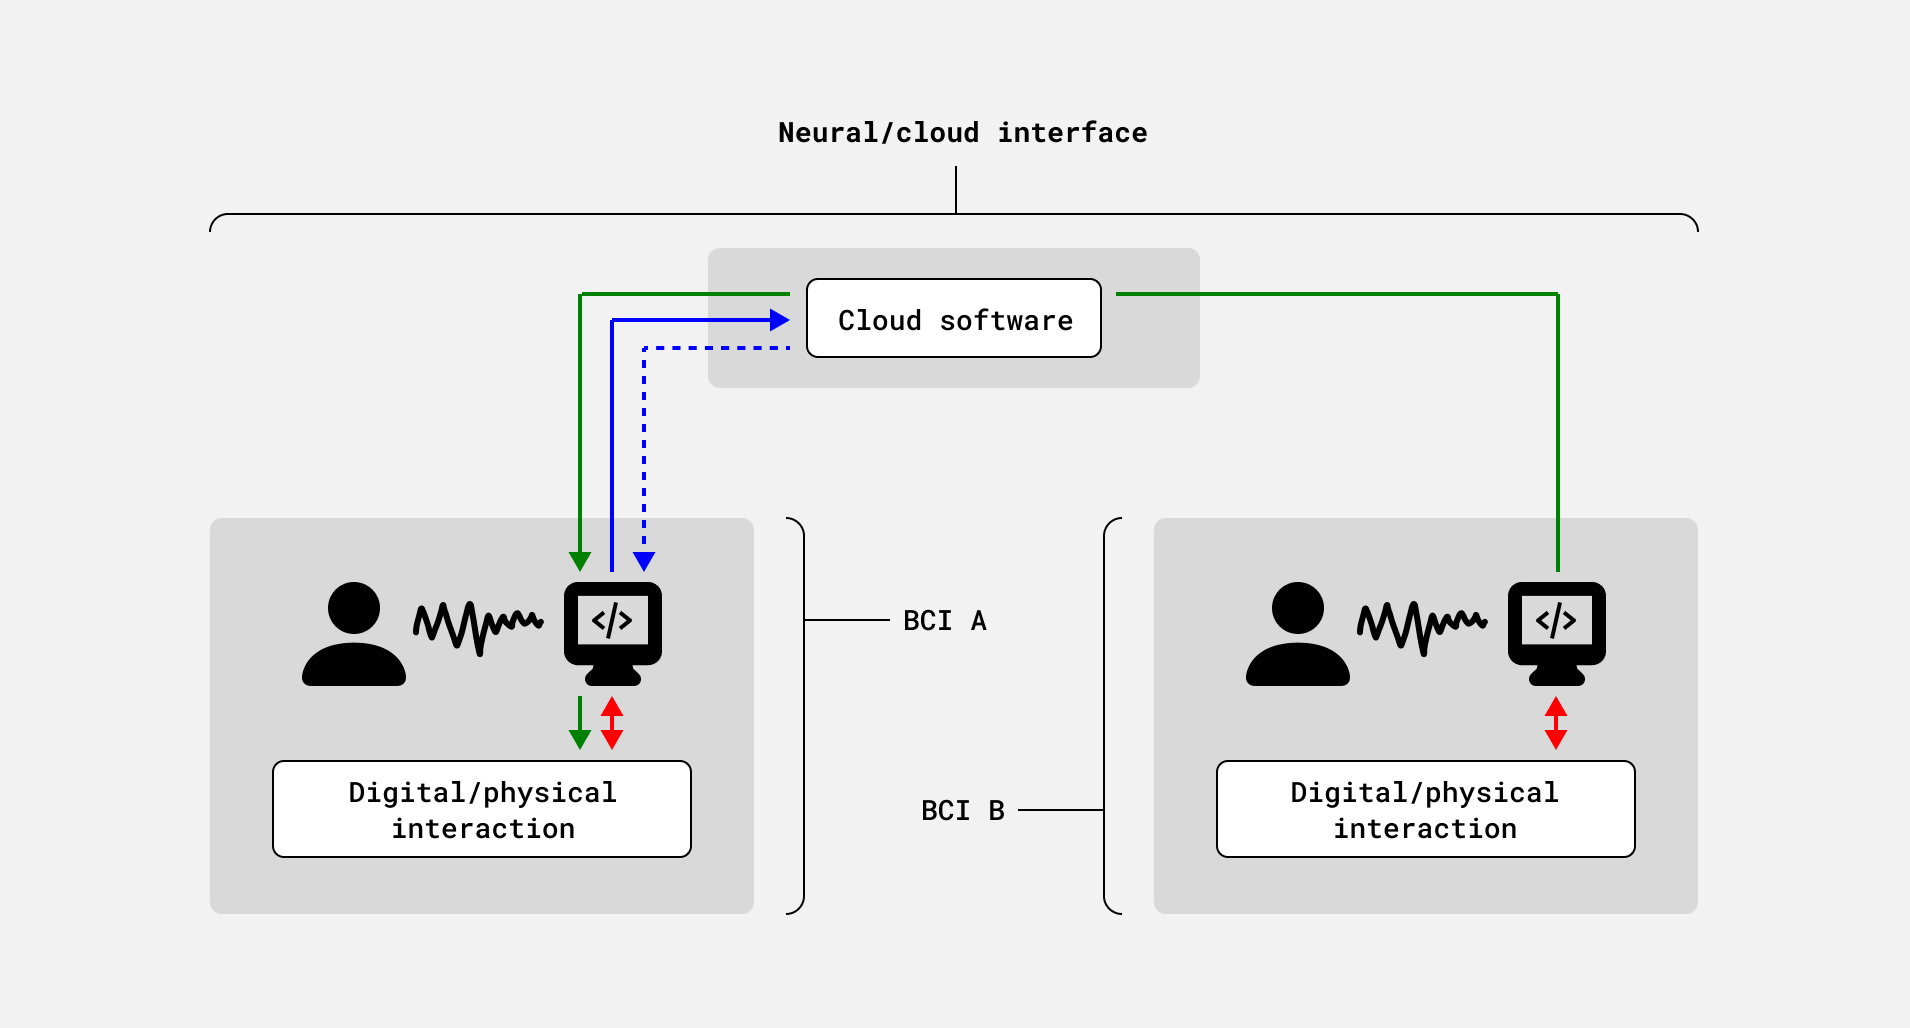
\includegraphics[width=\linewidth]{nci-overview.png}
  \caption{A N/CI is the connection between multiple BCIs.}
  \label{fig:nci-overview}
\end{figure}

\section*{Distinction between existing research}
\label{chapter2-distinction-between-existing-research}

The concept of running BCI software components remotely and on the cloud is not novel, as research into the concept known as asynchronous BCI \citep{an_design_2016} or internet-based BCI \citep{lampe_brain-computer_2014} has been ongoing for some time. However, when we look at the more recent research from \citeauthor{zhang_internet_2018} on their cloud-based deep learning framework to enable, as they describe Human-Thing Cognitive Interactivity, we see a strong emphasis on algorithms and machine learning but less on aspects such as the cloud architecture and mass-market-readiness \citep{zhang_internet_2018}. They address the latency and the size of EEG samples sent in near-real-time to a server, as well as the corresponding calculation, but there are no more details in regards to the proposed and very simplified architecture chart's components or effective cloud architecture, all of which factor into the author's aim to develop a N/CI. Another related and even more recent paper by \citeauthor{ahamad_system_2022} looks at the system architecture of a BCI for the Internet of Things (IoT), but this time from the perspective of algorithms optimised for time series data such as EEG, but still with no mention of the effective cloud architecture of such a system \citep{ahamad_system_2022}.

The author of this thesis introduces the concept of three-dimensionality for the definition of a N/CI based on the previously mentioned topics and research that touch on the issues of this thesis, which are essential to achieve general applicability for BCIs from the perspective of the software system for the actual implementation of such a system.

\section*{Requirements of a N/CI}
\label{chapter2-requirements-of-a-nci}

The term N/CI positions itself as a software system in the intersection that can undoubtedly be defined as production-grade rather than being in the PoC stage, unobtrusive implementation rather than obtrusive software and general-purpose applicability rather than being made just for a specific use case. \autoref{fig:nci-definition} illustrates the position of a N/CI within the mentioned properties. Subsequently, \autoref{tab:nci-axis} summarises the definitions as described in this thesis.

\begin{figure}[ht]
  \centering
  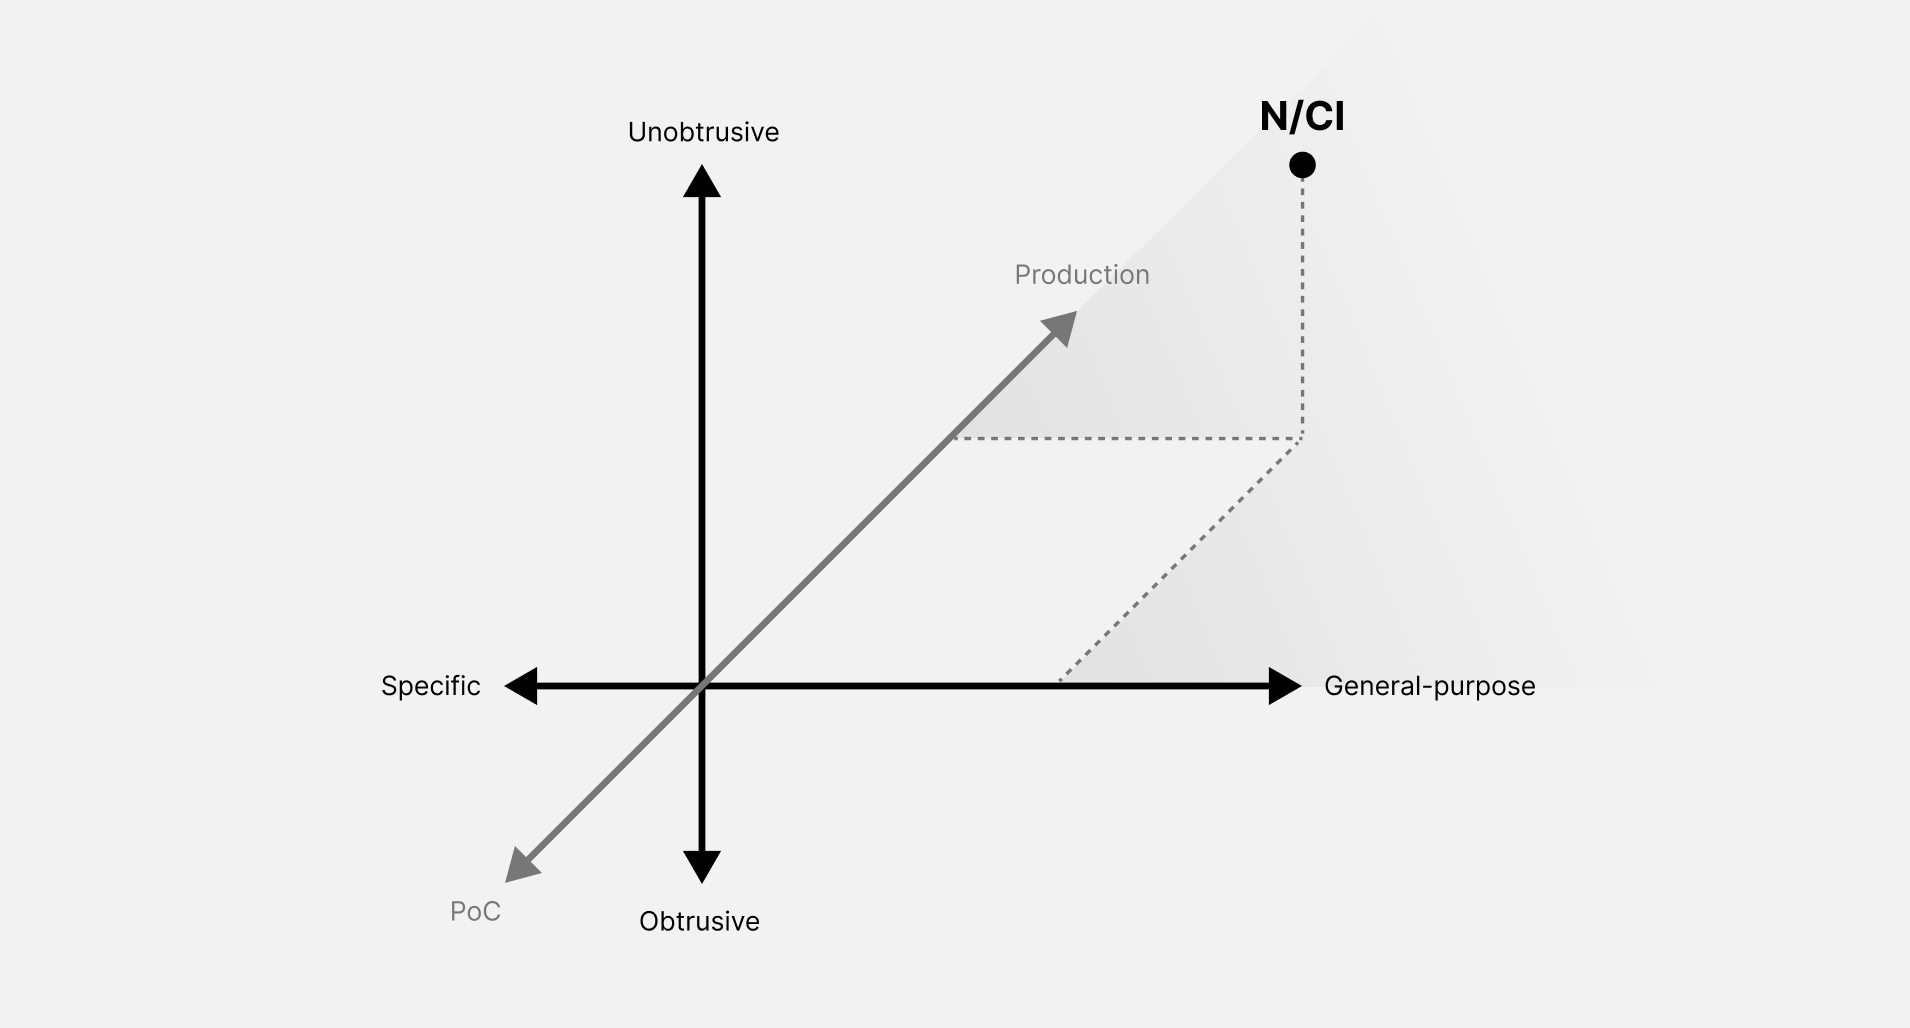
\includegraphics[width=\linewidth]{nci-definition.png}
  \caption{Visualisation of the three-dimensionality of the term neural/cloud interface with its three axes and differentiation of six terms.}
  \label{fig:nci-definition}
\end{figure}


\begin{landscape}
\begin{table}[ht]
  \centering
  \resizebox{\textwidth}{!}{%
    \begin{tabular}{ll}
      \rowcolor[HTML]{000000}
      {\color[HTML]{FFFFFF} Axis labelling}                   &
      {\color[HTML]{FFFFFF} Description}                                                                                                                                                                                                                                                                                                                                                                                                                                                                                                                                                                                  \\ \hline
      \multicolumn{1}{|l|}{\textbf{Production}}               &
      \multicolumn{1}{l|}{\begin{tabular}[c]{@{}l@{}}As previously stated, this is the range in which a software system is deemed ready for production.\\ Because the definition is vague, it is difficult to identify specific requirements that must be met for\\ a system to be considered production-ready. However, for a N/CI, this means running in a\\ production environment, e.g. in a cloud, on a real-world end-user server rather than, for example,\\ in a proof-of-concept environment such as in a lab.\end{tabular}}                                                                                     \\ \hline
      \multicolumn{1}{|l|}{\textbf{Unobtrusive}}              &
      \multicolumn{1}{l|}{\begin{tabular}[c]{@{}l@{}}As previously stated, an unobtrusive software system is one in which the end-user does not need\\ to understand the underlying architecture and requirements in order to use the software or even\\ know certain parts of the software system. In the reverse case, users need to install special\\ packages or download additional companion apps to make a N/CI work on their computer\\ or smartphone is not the aim of the author's definition of a N/CI.\end{tabular}}                                                                                          \\ \hline
      \multicolumn{1}{|l|}{\textbf{General-purpose}}          &
      \multicolumn{1}{l|}{\begin{tabular}[c]{@{}l@{}}A general-purpose software system is one that can be used for a variety of functions. As an\\ example, consider AWS. It is general-purpose, which means that developers can create\\ cloud software on AWS that can be either a financial application or a backend for a mobile\\ game; there are no specific use cases. This means that a N/CI, unlike the NextMind BCI\\ or the Muse headband, should provide general-purpose functionality rather than specific use\\ cases, i.e. it is not limited to a specific set of functions.\end{tabular}}                 \\ \hline
      \rowcolor[HTML]{EFEFEF}
      \multicolumn{1}{|l|}{\cellcolor[HTML]{EFEFEF}PoC}       &
      \multicolumn{1}{l|}{\cellcolor[HTML]{EFEFEF}\begin{tabular}[c]{@{}l@{}}A BCI software system that serves as a proof of concept cannot be considered N/CI because\\ it is not intended for production and thus all the effort required to create a production system,\\ such as quality assurance with unit or end-to-end testing, is unnecessary. A PoC system does\\ not usually run in a production environment, as the goal is, for example, to test a specific\\ functionality of a use case rather than to deliver the software to end-users.\end{tabular}}                                                    \\ \hline
      \rowcolor[HTML]{EFEFEF}
      \multicolumn{1}{|l|}{\cellcolor[HTML]{EFEFEF}Obtrusive} &
      \multicolumn{1}{l|}{\cellcolor[HTML]{EFEFEF}\begin{tabular}[c]{@{}l@{}}An obtrusive BCI system, for example, may still be production-ready if it targets specific use cases\\ while remaining unobtrusive because neuroscientists or developers, for example, expect to have\\ access to the underlying software architecture or technical requirements and thus do not want to\\ abstract from it. If it is obtrusive software, such as OpenBCI, this usually means building the\\ production-ready part on top of it is necessary, which does not fit the author's proposed definition\\ of a N/CI.\end{tabular}} \\ \hline
      \rowcolor[HTML]{EFEFEF}
      \multicolumn{1}{|l|}{\cellcolor[HTML]{EFEFEF}Specific}  &
      \multicolumn{1}{l|}{\cellcolor[HTML]{EFEFEF}\begin{tabular}[c]{@{}l@{}}If a BCI system is only used for one use case, such as Muse for sleep and meditation, companies\\ or developers who want to offer a different use case, such as a mind-controlled keyboard with a\\ P300 system will have to reverse engineer Muse's EEG output or use a different BCI hardware\\ that is less specific and closed, and then build their own production-ready and unobtrusive software\\ on top of it.\end{tabular}}                                                                                                         \\ \hline
    \end{tabular}%
  }
  \vspace{10pt}
  \caption{Axes label descriptions of the three-dimensionality for the definition of a N/CI as shown on \autoref{fig:nci-definition}.}
  \label{tab:nci-axis}
\end{table}
\end{landscape}

\newpage

With an unobtrusive form factor like the one developed by IDUN Technologies, a significant hardware barrier to becoming a mass-market BCI has already been tackled. Next to the hardware, IDUN intends to provide a business-to-business (B2B) software platform, allowing 3rd-party developers to create software on top of IDUN's offerings through a universal brain application programming interface (API). Because they allow others to consume this API in end-user-facing apps, it must be production-ready and unobtrusively able to be integrated. IDUN's hardware and software aim to be general-purpose rather than specific, allowing others to build any BCI-enhanced app \citep{idun_guardian_nodate}.

All of IDUN's requirements systematise one of the first BCI aimed at the general public, which satisfies the broad definition of a N/CI. The fundamental motivation of the author is to standardise collaboration and research on this novel and interdisciplinary field of BCI software and cloud computing.
